\documentclass{beamer}
\usetheme{Hannover}


\usepackage{algorithm}
\usepackage{algorithmic}
\usepackage{amsmath}
\usepackage{amssymb}
\usepackage{amsthm}
\usepackage[ngerman,english]{babel}
\usepackage{centernot} 
\usepackage{color}
\usepackage{dsfont}
\usepackage{graphicx}
\usepackage[utf8]{inputenc}
\usepackage{import}
\usepackage{standalone}
\usepackage{qtree}

\usepackage{hyperref}

\title{Integral infeasibility and testing total dual integrality}
\author{David L.Applegate, William Cook S.Thomas McCormick}

\newcommand{\N}{\ensuremath{\mathds{N}}}
\newcommand{\R}{\ensuremath{\mathds{R}}}
\newcommand{\red}[1]{\textcolor{red}{#1}}

\setlength{\itemsep}{-2pt}


\begin{document}

%%%%%%%%%%%%%%%%%%
%%%%%%    %%%%%%%%
%%%%%%%%%%%%%%%%%%



%%%%%%%%%%%%%%%%%%
%%%%%%    %%%%%%%% stronger linear systems
%%%%%%%%%%%%%%%%%%

\begin{frame}{Integral Infeasibility}

	\begin{block}{Variations of the Linear System}

		For a system $Ax \leq b$ of $m$ linear inequalities and a set $T\subset \{1, \dots, m \}$ and $\bar{T} = \{1, \dots, m \} \setminus T$, we let
		\begin{equation}\label{eq:2}
		A_T x = b_T, A_{\bar{T}} x \leq b_{\bar{T}} 
		\end{equation} 
		denote the system obtained by settig each inequality in T to equality. 

	\end{block}

\end{frame}



\begin{frame}  % important theorems for proofs

	% \begin{block}{Complementary Slackness}

	% 	Let $x_0$ and $y_0$ be feasible solutions in the primal and dual problem respectively.
	% 	That is, $Ax_0 \leq b$ and $y_0 A = w; y_0 \geq 0$. \\
	% 	Then $w x_0 = y_0 b$ iff. $(y_0)_i > 0  \Rightarrow A_i x_0 = b_i$

	% \end{block}	

	\begin{block}{Farkas Lemma}

		For $A \in \mathbb{R}^{m \times n}, b \in \mathbb{R}^{m}$ then exactly one of the following is true: \\
		1. There exists $x \in \mathbb{R}^n$ such that $Ax \leq b$. \\
		2. There exists $y \in \mathbb{R}^m$ such that $yA=0, yb<0$ and $y \geq 0$. 

	\end{block}

	\begin{block}{Note}

		Furthermore, in relation to Farkas Lemma, we have that exactly one of the following is true: \\
		1. There exists $x \in \mathbb{R}^n$ such that $Ax=b$. \\
		2. There exists $y \in \mathbb{R}^m$ such that $yA=0$ and $by \neq 0$.


	\end{block}

\end{frame}

%%%%%%%%%%%%%%%%%%
%%%%%%    %%%%%%%% Infeasibility by Farkas
%%%%%%%%%%%%%%%%%%

\begin{frame}

	\begin{block}{Infeasibility realtion}

		With the use of Farkas lemma for $A_{\bar{T}} x \leq b_{\bar{T}}$ and the observation for $A_T x = b_T$ we see that the system $A_{\bar{T}} x \leq b_{\bar{T}}$, $A_T x = b_T$ is not feasible if there exists a vector $(y_T, y_{\bar{T}})$ such that\\

		\begin{eqnarray}\label{eq:3}
			y_T b_T + y_{\bar{T}} b_{\bar{T}} & < & 0 \nonumber\\
			y_T A_T + y_{\bar{T}} A_{\bar{T}} & = & 0 \nonumber\\
			y_{\bar{T}} \geq 0.
		\end{eqnarray}

	\end{block}

\end{frame}

\begin{frame}

	\begin{block}

		Values of $y_T$ can possibly be negative due to equality constraints. Due to scaling we can still pose the constraints

		\begin{eqnarray} \label{eq:4}
			y_T b_T + y_{\bar{T}} b_{\bar{T}} & < & 0 \nonumber\\
			y_T A_T + y_{\bar{T}} A_{\bar{T}} & = & 0 \nonumber\\
			y_T \geq -1 & y_{\bar{T}} \geq 0.
		\end{eqnarray}

		By construction of the linear system, this now gives us, with the use of Farkas Lemma and the observation, that if such a vector exists the system $A_{\bar{T}} x \leq b_{\bar{T}}$, $A_T x = b_T$ has not feasible solution. This result is used in the upcomming Theorem.

	\end{block}

\end{frame}

%%%%%%%%%%%%%%%%%%
%%%%%%    %%%%%%%%
%%%%%%%%%%%%%%%%%%

\begin{frame}{Definitions}

	\begin{block}

		We say that the \textbf{infeasibility} of (\ref{eq:2}) can be \textbf{proven integrally} if (\ref{eq:4}) does in fact have an integral solution. 

	\end{block}

	\begin{block}{Hilbert basis}

		A set of vectors $\{h_1, \dots, h_k\}$ is called Hilbert basis if each integral vector in the cone $C(\{h_1, \dots, h_k\}) :=$\\ $\{\sum_{i\in \{ 1,\dots,k \}} \lambda_i h_i; \lambda_i \geq 0$ for all $i \in \{1,\dots,k\} \}$ can be written as integral combination of $h_1, \dots, h_k$.

	\end{block}

\end{frame}


%%%%%%%%%%%%%%%%%%
%%%%%%    %%%%%%%%
%%%%%%%%%%%%%%%%%%

\begin{frame}

	\begin{block}{Theorem 1}

		Let $A\in \mathbb{Z}^{m \times n}$ and $b$ a rational vector such that the linear system $Ax \leq b$ has at least one solution. Then $Ax \leq b$ is totally dual integral \textbf{if and only if}\\

		\begin{enumerate}[i]

			\item the rows of $A$ form a Hilbert basis, and

			\item for each subset $T$ of inequalities from $Ax\leq b$, if (\ref{eq:2}) is infeasible, then this can be proven interally.

		\end{enumerate}

	\end{block}

	\begin{block}{Reminder - (\ref{eq:2})}

		For $T\subset \{ 1, \dots, m\}, \bar{T} = \{1, \dots, m \} \setminus T$ the system (\ref{eq:2}) was given by $A_T x= b_T$ and $A_{\bar{T}}x\leq b_{\bar{T}}$.

	\end{block}

\end{frame}


% \begin{frame}{Proof}
	
% 	\begin{block}{"$\Leftarrow$""}  %% make proof sketch!!
% 		\small
% 		Suppose $Ax\leq b$ has a solution and (i) and (ii) hold. For $w\in \mathbb{Z}^n$ such that a the optima for $max\{wx:Ax\leq b\}=min\{yb: yA=w, y\geq 0 \}$. We show that the right-hand side has an integral optimal solution.\\

% 		Since the rows of A form a Hilber basis we find a solution $y^*$ chosen such that $y^* b$ is as small as possible. Choose T such that $(y^*)_i>0$ for $i\in T$. Now if the system $A_T x= b_T$, $A_{\bar{T}}x\leq b_{\bar{T}}$ is feasible, then by complementary slackness (see next slide), $y^*$ is optimal. Otherwise, by (ii) we know that there exists an integral solution $\bar{y}$ for (4). From this follow, since $y_T^* > 0$, $y^* + \bar{y}$ is a solution to (6) for which $(y^*+\bar{y})b < y^* b$ and therefore a contradiction. $y^*$ must be optimal integral solution to (6).

% 	\end{block}

% \end{frame}

% \begin{frame}

% 	\begin{block}{"$\Rightarrow$"}



% 	\end{block}

% \end{frame}

% reminder

% \begin{frame}  % important theorems for proofs

% 	\begin{block}{Complementary Slackness}

% 		Let $x_0$ and $y_0$ be feasible solutions in the primal and dual problem respectively.
% 		That is, $Ax_0 \leq b$ and $y_0 A = w; y_0 \geq 0$. \\
% 		Then $w x_0 = y_0 b$ iff. $(y_0)_i > 0  \Rightarrow A_i x_0 = b_i$

% 	\end{block}	

% \end{frame}

%%%%%%%%%%%%%%%%%%
%%%%%%    %%%%%%%% Faces
%%%%%%%%%%%%%%%%%%

\begin{frame}{Testing for total dual inegrality}

	\begin{block}{Test by Cook, Lovász and Schrijver} 

		Cook, Lovász and Schrijver (source) developed a polynomial-time test  (for fixed dimension) for the total dual integrality. \parskip=15pt

		Based on the fact that \\
		$Ax\leq b$ is totally dual integral \textbf{if and only if} for each minimal face $F_J$ the set of active rows form a Hilbert basis.
		\parskip=15pt
		
		Can be checked with Lenstra's integer programming algorithm. Number of times is exponential in with respect to the dimension. Not praktical for application.

	\end{block}
		
\end{frame}


\begin{frame}

	\begin{block}{Faces; minimal Faces}

		For $P\subset \mathbb{R}^n$ a polyhedron given by $Ax\leq b$, $J\subset \{1,\dots , m\}$, define $F_J := \{x \in P | a_i x = b_i$ for $i \in J\}$ as a Face of P.\\
		A minimal Face of $P$ does not contain another Face.

	\end{block}

	\pause

	% Beispiel RB Tree
	\begin{figure}[htp]
		\centering
		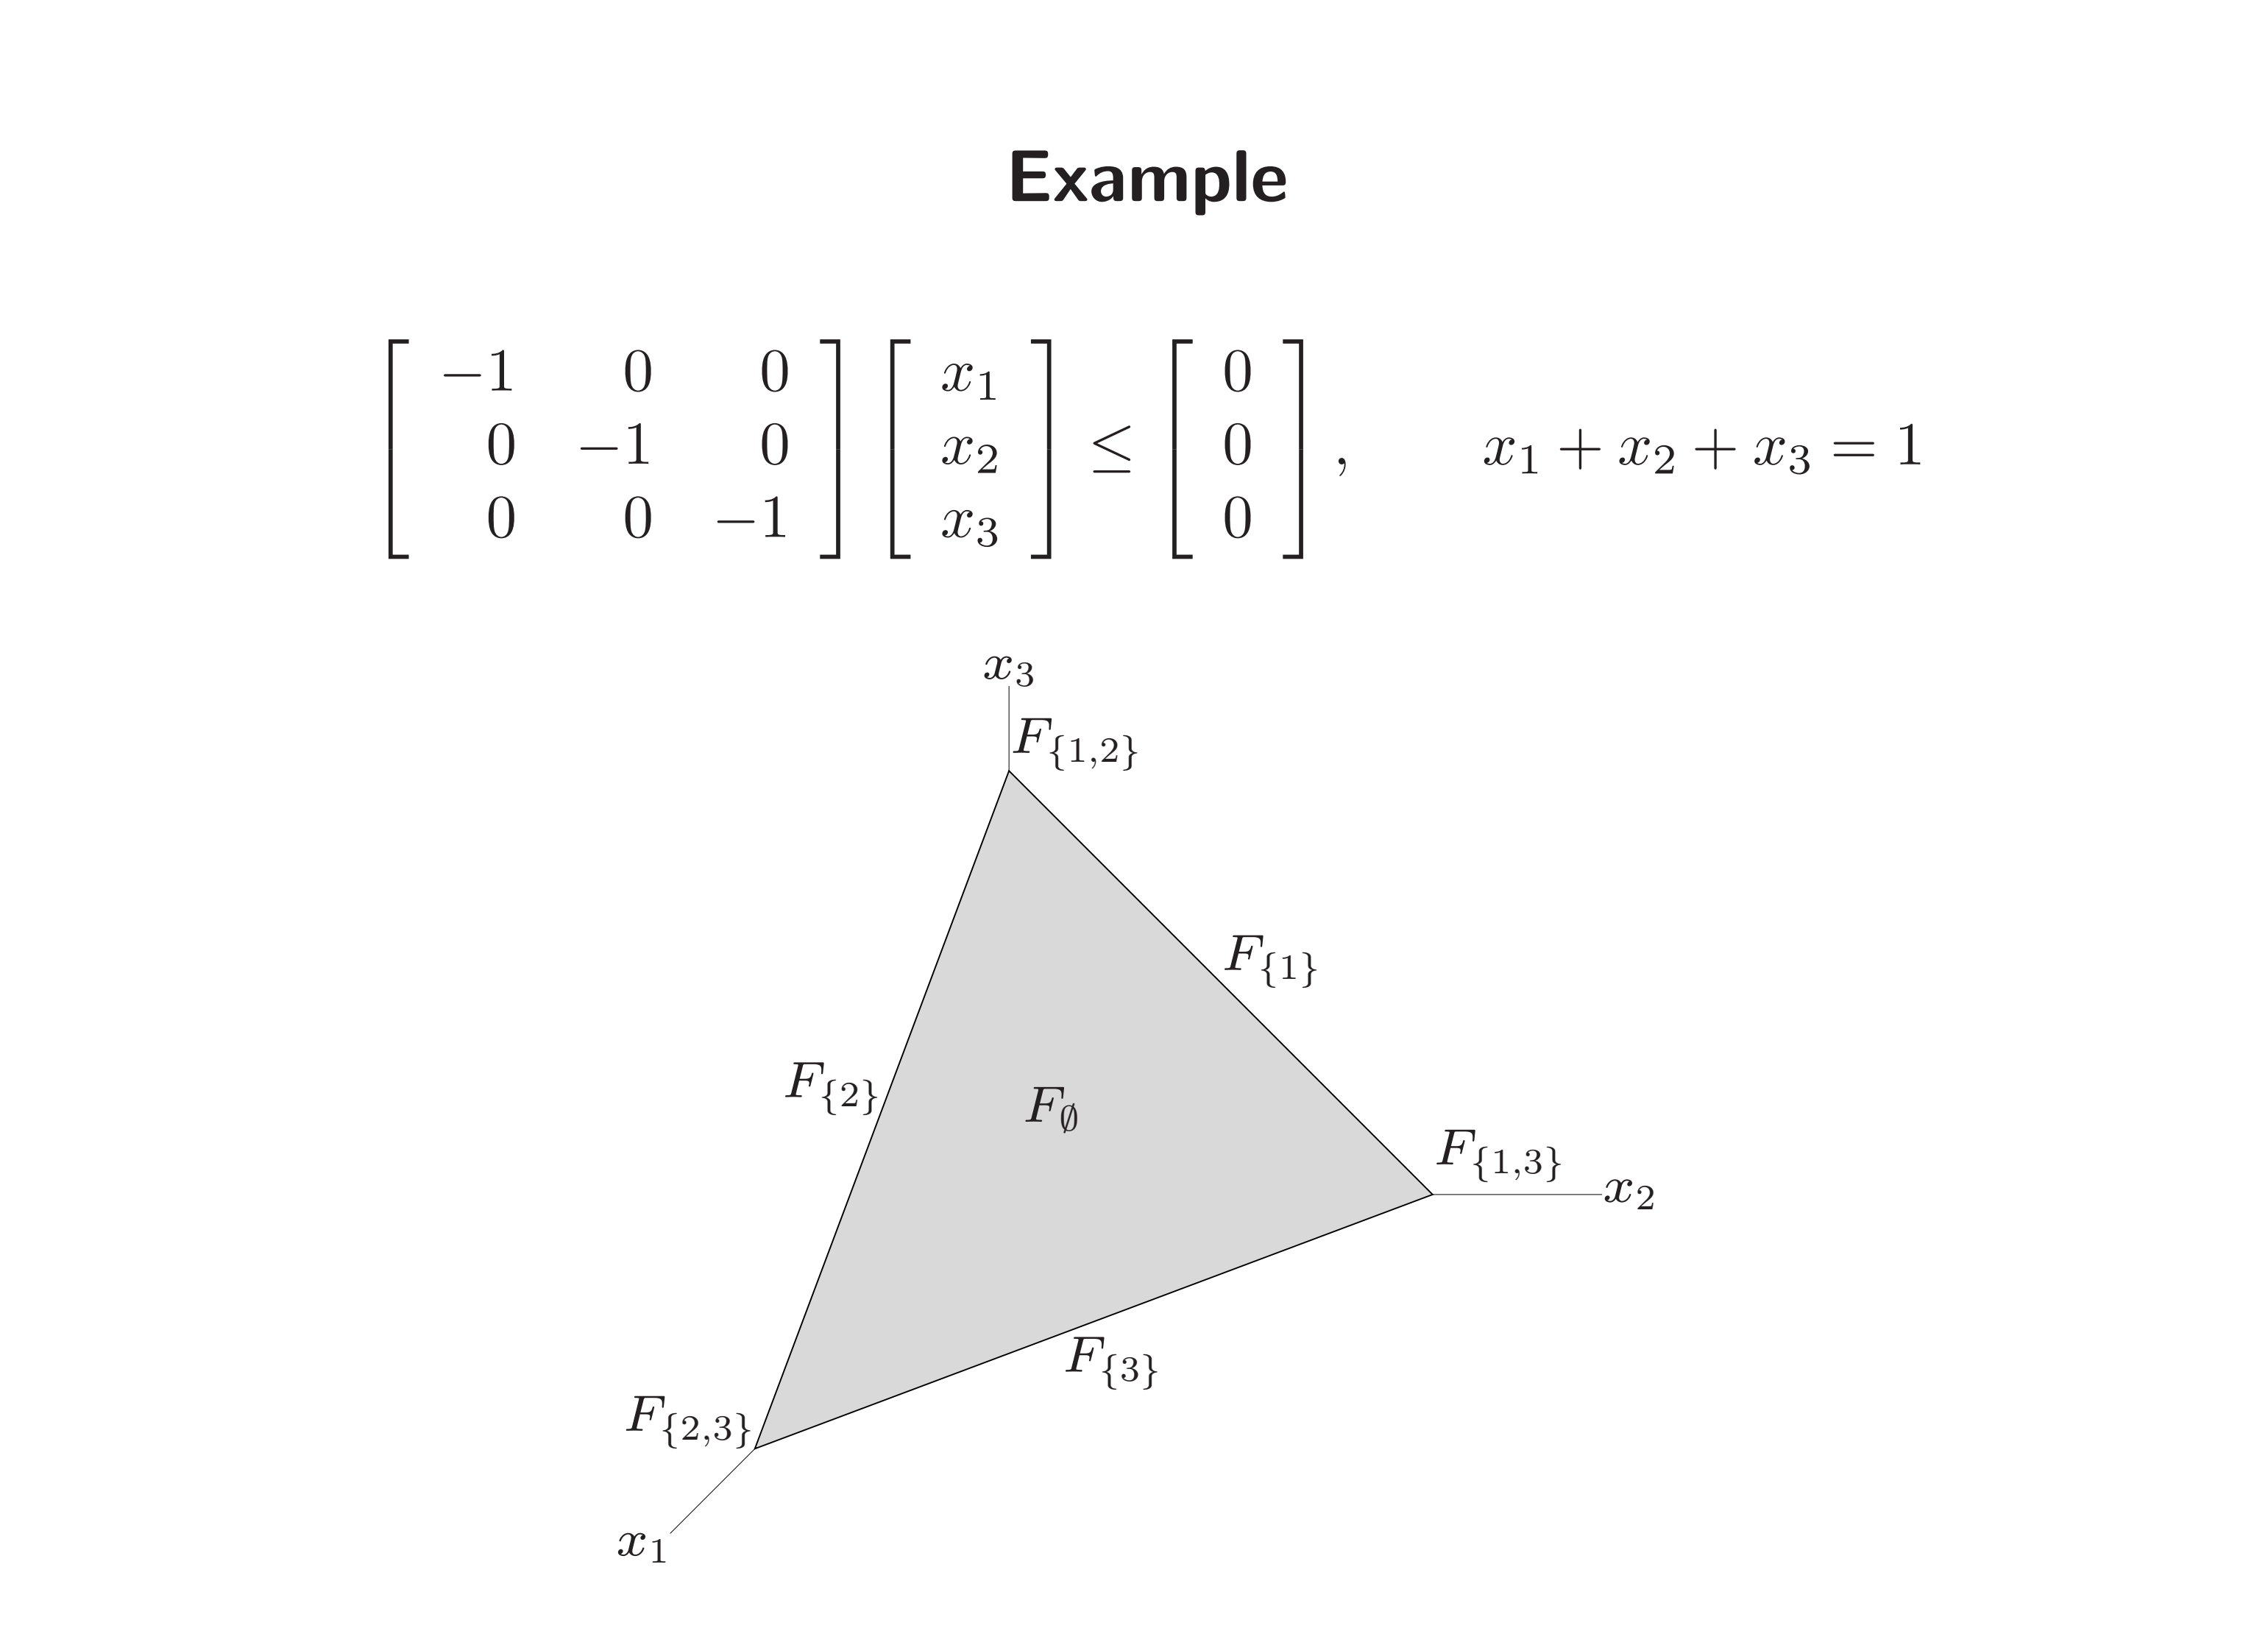
\includegraphics[width=6cm]{images/faces_example.png}
		\caption{http://www.seas.ucla.edu/~vandenbe/ee236a/lectures/polyhedra.pdf}
		\label{fig:faces_example}
	\end{figure}

\end{frame}

% \begin{frame}
% 	\frametitle{Example Faces}
	
% 	% Beispiel RB Tree
% 	\begin{figure}[htp]
% 		\centering
% 		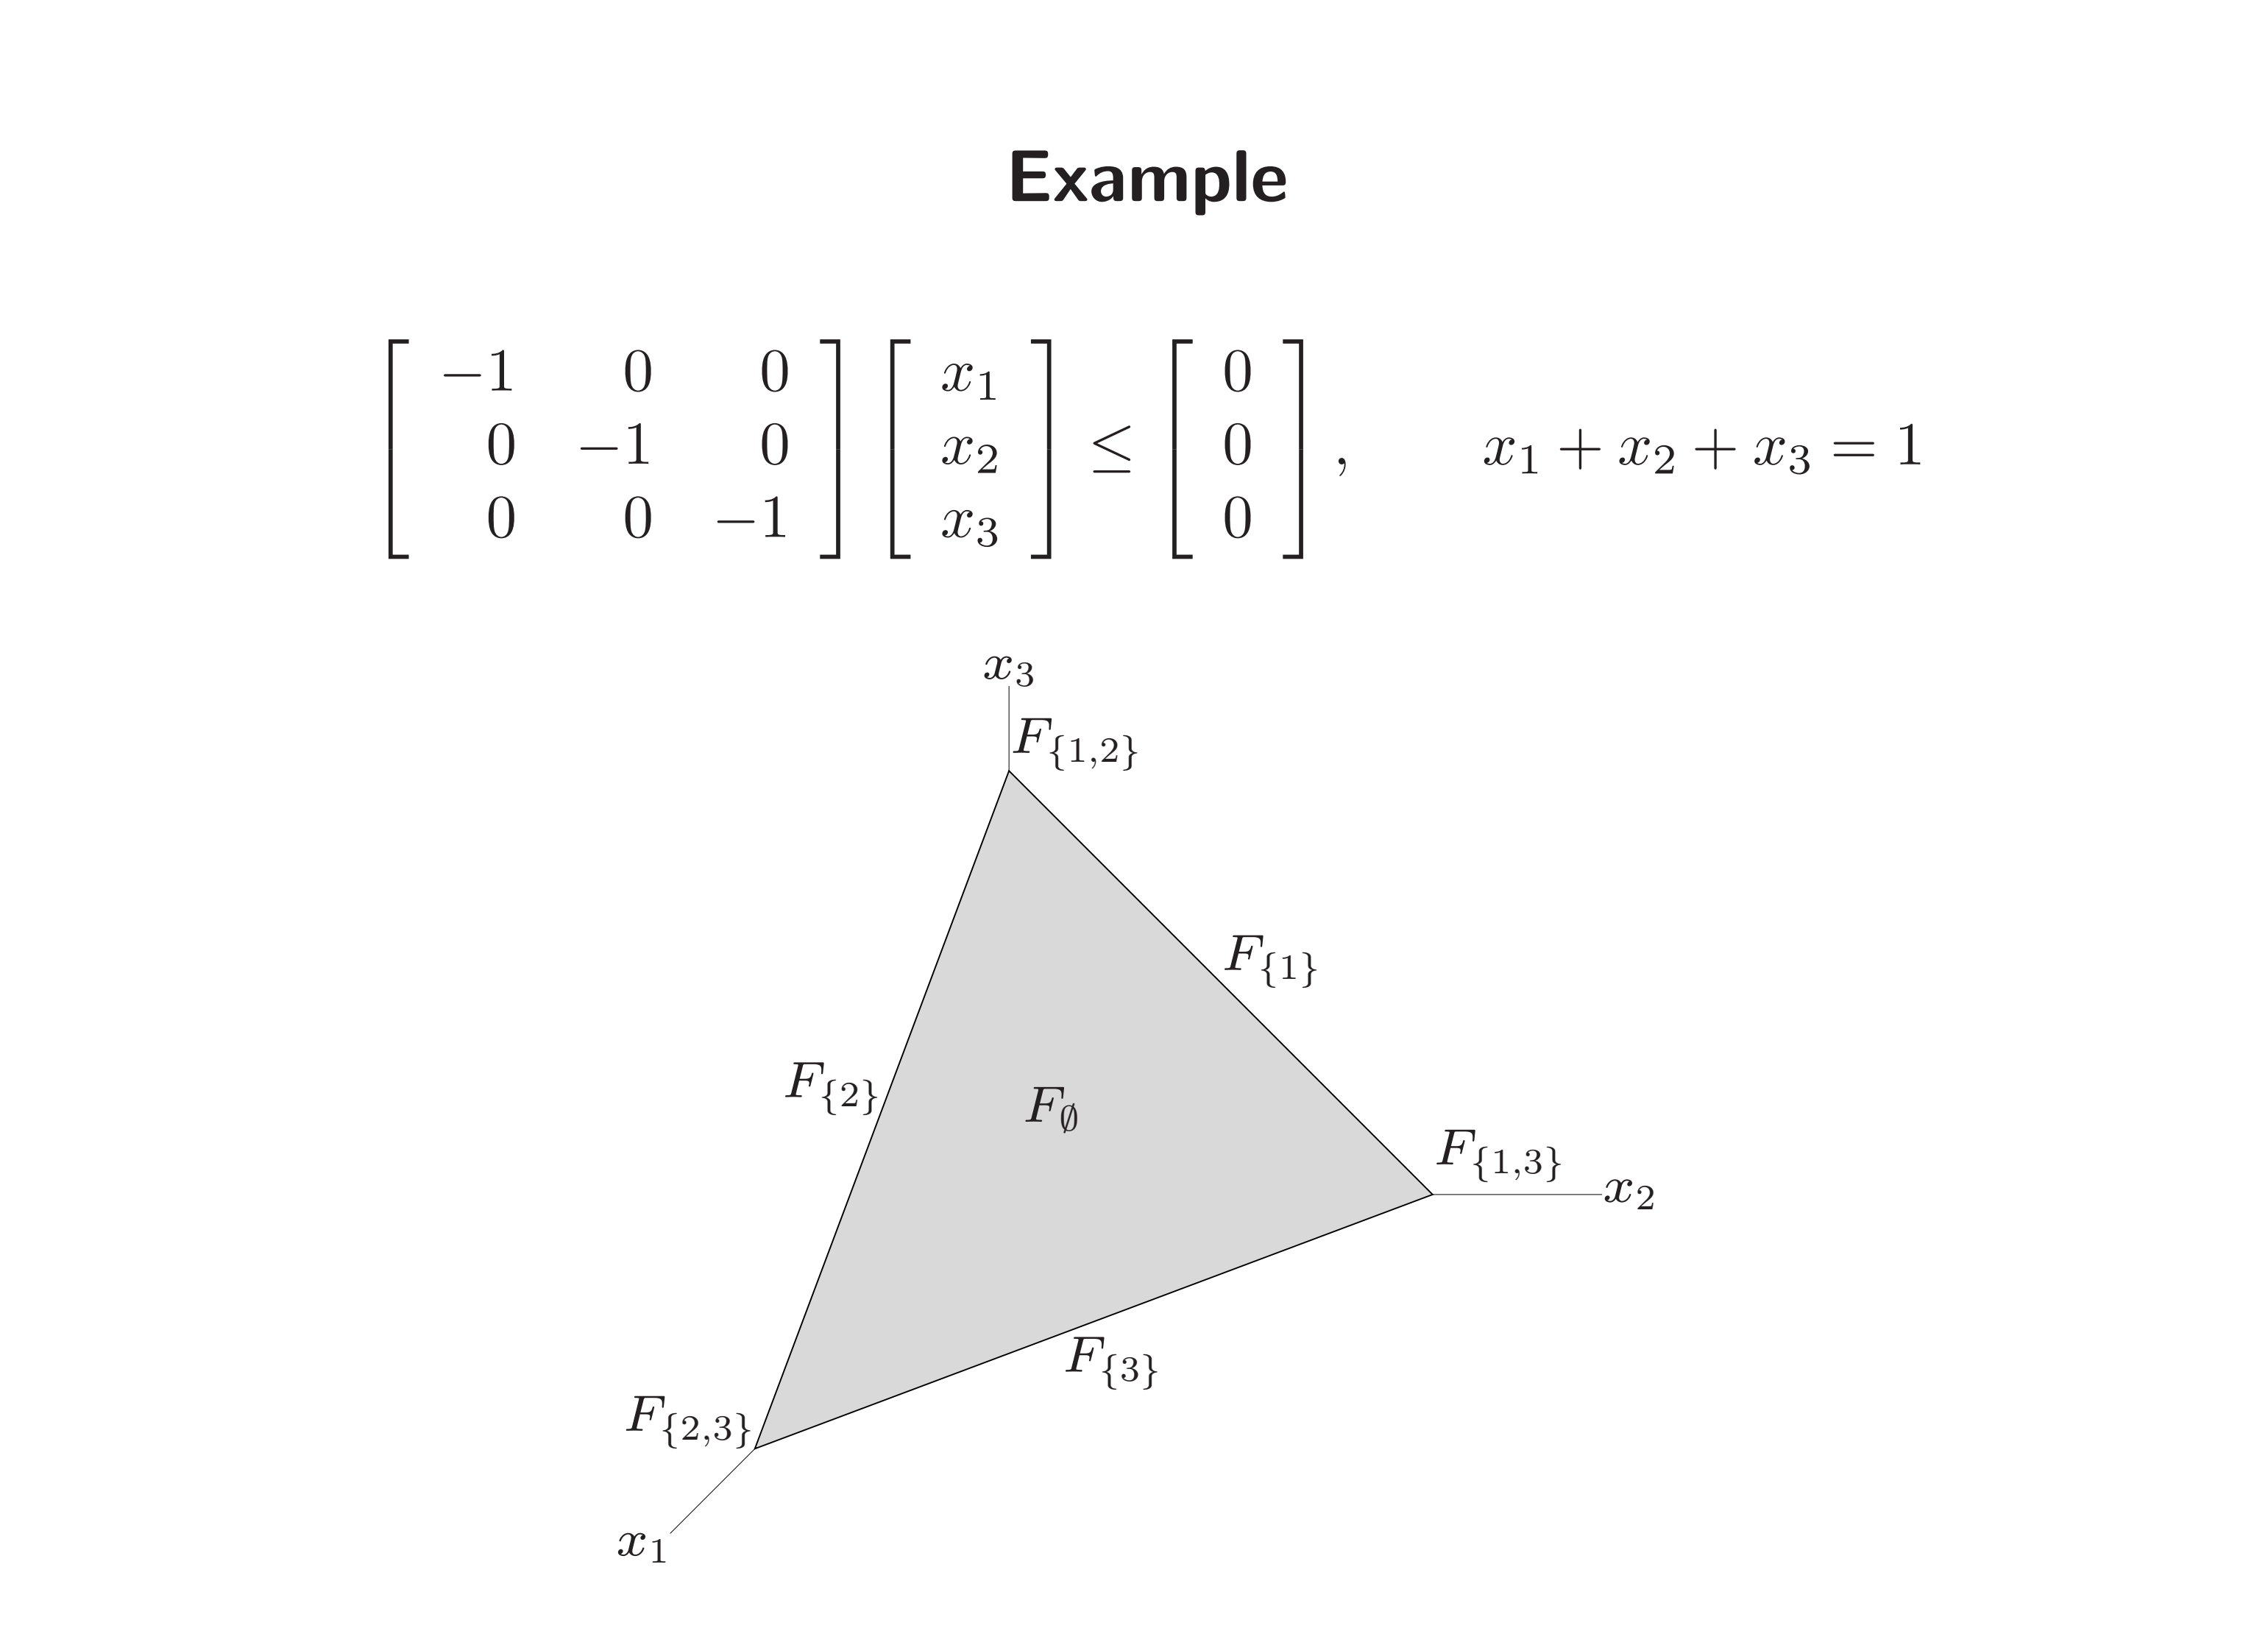
\includegraphics[width=8cm]{images/faces_example.png}
% 		\caption{http://www.seas.ucla.edu/~vandenbe/ee236a/lectures/polyhedra.pdf}
% 		\label{fig:faces_example}
% 	\end{figure}
% \end{frame}



%%%%%%%%%%%%%%%%%%
%%%%%%    %%%%%%%% Theorem 2
%%%%%%%%%%%%%%%%%%


\begin{frame}

	\begin{block}

		It is of practical interest to avoid Hilber basis tests whenever possible. Thus Theorem 2 helps in certain cases.

	\end{block}

	\pause

	\begin{block}{Theorem 2}

		Let $A\in \mathbb{Z}^{m \times n}$ and $b$ a rational vector such that the linear system $Ax \leq b$ has at least one solution. Then $Ax \leq b$ is totally dual integral \textbf{if and only if}\\

		\begin{enumerate}[i]

			\item the rows of $A$ form a Hilbert basis, and

			\item for each subset $T$ of at most $n$ inequalities from $Ax\leq b$, the linear programming problem \\
			$min\{yb: yA=1\cdot A_T, y\geq 0 \}$ has an integral solution.

		\end{enumerate}

	\end{block}

\end{frame}

\begin{frame}

	\begin{block}{Improvements} 

		\begin{itemize}

			\item integer programming problems of the form \begin{equation*} min \{yb: yA=w, y\geq 0 \}\end{equation*} for totally dual integral systems $Ax \leq b$ ($A, w$ integral) are solvable in polynomial time (Chandrasekaran, Schrijver)

			\item sometimes checking of condition (i) is possible without using the test of Cook, Lovász and Schrijver

		\end{itemize}

	\end{block}

\end{frame}


\end{document}
